\chapter{Descrizione UML} \label{cap}
\def\baselinestretch{1.66}

Seguendo il diagramma UML delle classi spieghiamo come \`{e} stato sviluppato il software.\\

\section{Factory Pattern}
L'accesso pu\`{o} avvenire in modalit\`{a} utente o in modalit\`{a} amministratore, a tal proposito \`{e} stato utilizzato un \textbf{factory pattern}, il metodo Accedi della classe Login \`{e} implementato dalle classi Utente e Amministratore per controllare le credenziali di accesso in due differenti tabelle. \\
\begin{center}
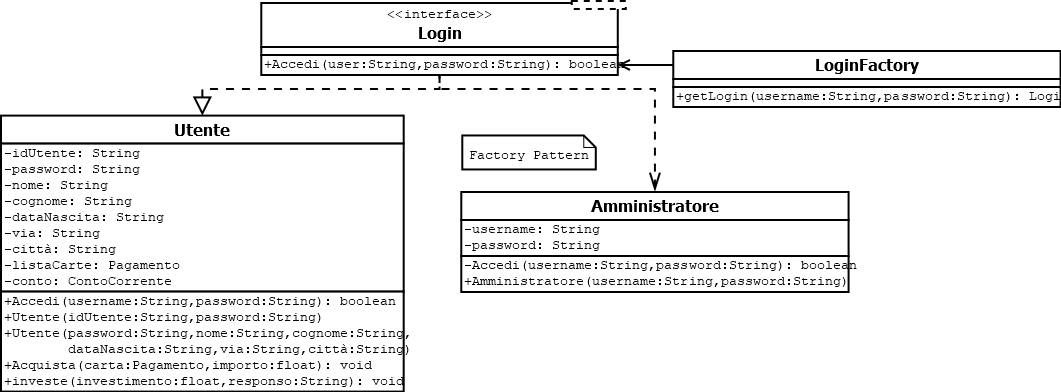
\includegraphics[scale=0.40]{FactoryPattern.png}
\end{center}

\section{Chain of Responsibility}
Proseguendo la lettura del diagramma in direzione dell'Amministratore, il pattern \textbf{CoR} definisce una classe astratta Investimento e le classi concrete BassoRischio, MedioRischio e AltoRischio che applicano una diversa logica al metodo investi.\\
La conclusione del pattern \`{e} nella servlet EffettuaInvestimento che data una stringa da alla prima classe della catena la richiesta che seguir\`{a} poi fino a trovare chi pu\`{o} soddisfare la richiesta. \\
\begin{center}
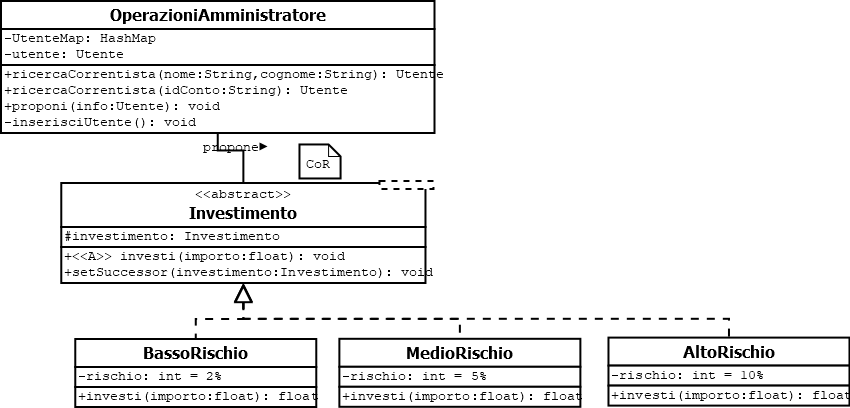
\includegraphics[scale=0.40]{CoR.png}
\end{center}

\section{Template Method}
Passando alla parte dello schema riguardante l' utente, il primo pattern \`{e} \textbf{TemplateMethod} il quale \`{e} stato pensato per astrarre il comportamento dei metodi versa e preleva che sono implementati dalle classi ContoBasic, ContoMedium, ContoPremium fornendo l'implementazione dei restanti metodi che risulteranno comuni per i vari tipi di conto corrente.\\
\begin{center}
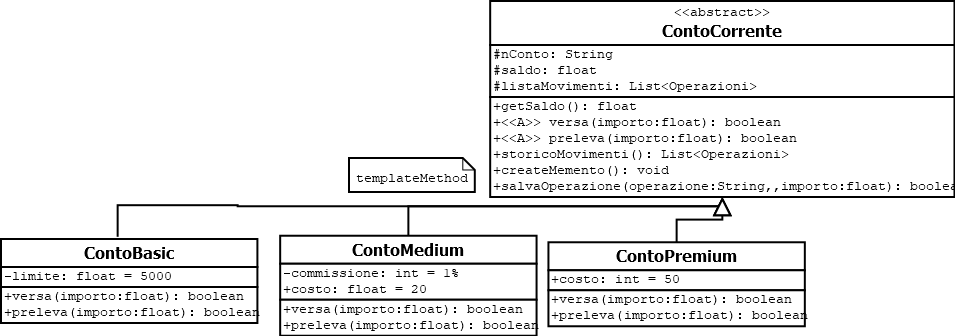
\includegraphics[scale=0.40]{TemplateMethod.png}
\end{center}

\section{Memento}
Il pattern \textbf{Memento} permette all'utente di poter annullare l'ultimo acquisto effettuato tramite carta di credito. \\
\begin{center}
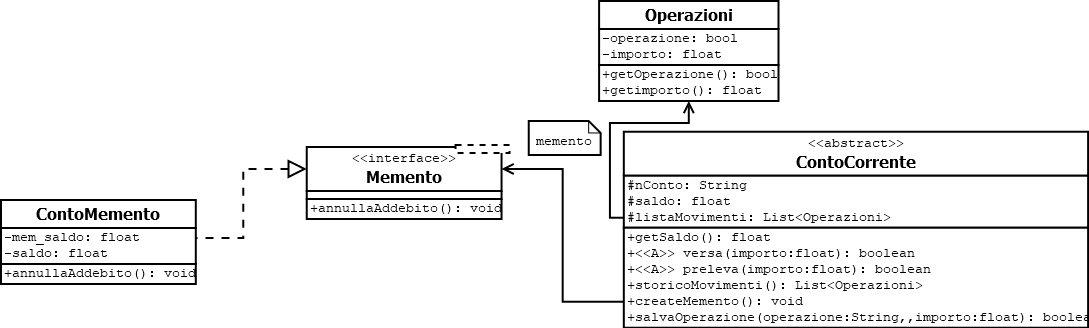
\includegraphics[scale=0.40]{Memento.png}
\end{center}

\section{Strategy}
L' utente pu\`{o} effettuare un acquisto con carta di credito o con carta prepagata, il pattern \textbf{strategy} consente di implementare due strategie di pagamento differenti, nel primo caso viene applicata la logica di pagamento relativa al tipo di conto corrente posseduto, nel secondo controllando il saldo della carta prepagata.\\
\begin{center}
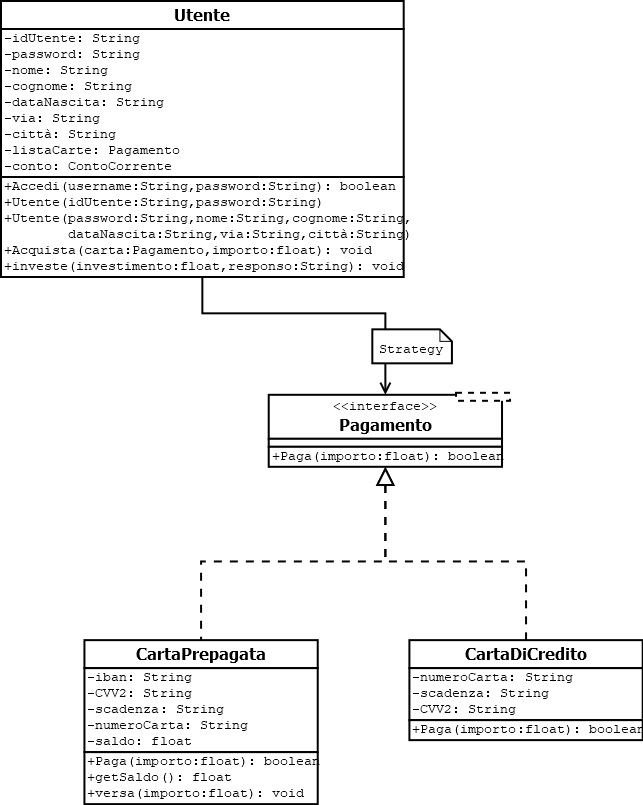
\includegraphics[scale=0.40]{Strategy.png}
\end{center}

\section{Decorator}
La possibilit\`{a} di aggiungere uno sconto a run-time al proprio conto corrente \`{e} realizzata mediante il pattern \textbf{decorator}. In base al codice sconto iserito, l'utente riceve un diverso tipo di codice sconto, viene dunque decorato l'oggetto relativo al proprio conto corrente.\\
\begin{center}
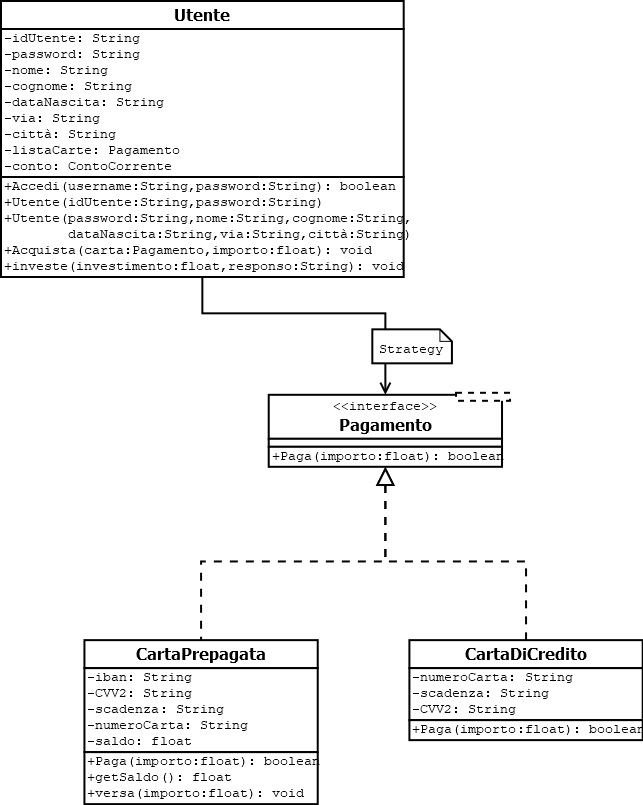
\includegraphics[scale=0.40]{Strategy.png}
\end{center}

Il pattern \textbf{singleton} \`{e} usato in diversi contesti per mantenere un unica istanza dell' oggetto contoCorrente, in modo che essa possa essere eventualmente decorata.\\

 